\documentclass[a4paper]{article}	% list options between brackets
\usepackage{}             		 % list packages between braces
\usepackage{url}
\usepackage{listings}
\usepackage{graphicx}
\usepackage{color}
\usepackage{enumitem}

% type user-defined commands here

\begin{document}

\begin{titlepage}
\title{\Huge \bfseries Sorting Criteria and ... \vspace{3 mm}\\ \Large \normalfont Subtask 5 - RSD1 Robot System Design\vspace{10mm}}   % type title between braces
\author{Martin Moghadam, Kalle Grafstr\"{o}m, \\ Audrius Palisaitis and Robertas Jacauskas}         % type author(s) between braces
\maketitle

\begin{abstract}
RSD1 Project
\end{abstract}

\end{titlepage}

%=======================================

\setcounter{page}{1}
\pagenumbering{roman}

\newpage
\tableofcontents
\newpage

\setcounter{page}{1}
\pagenumbering{arabic}

% Intro section
\section{Introduction}

The report documents the project of subtask 5 in the course RSD, Robot System Design.

\subsection{Project Description}

The the beginning of the course we were handed a description of subtask 5:

\begin{itemize}
\item Task description
	\begin{itemize}
	\item Everybody knows that washing black and white together is a bad idea, but there are a lot more criteria to consider, to prepare a wash
		\begin{itemize}
		\item Appropriate colors for joint was
		\item Washing conditions - e.g. temperature, centrifugation, spinning speed, drying
		\end{itemize}
	\item The appropriate amount of laundry should be prepared in piles or containers, which correspond to the load size of a washing machine
	\item When elders move in their clothes will be tagged (subtask 6), but the washing recipes of each item should also be registered
		\begin{itemize}
		\item That task should be simple for the staff
		\end{itemize}
	\end{itemize}
\item Challenges
	\begin{itemize}
	\item Together with group of subtask 6 create an easy an appropriateinterface for registering clothes and washing recipes
	\item Control criteria for the robot arm in subtask 4
	\item Close collaboration with subtask 4 and 6
	\item Perhaps some “untagged” clothes shouldbe put in washing bags?
	\end{itemize}
\item Technologies available
	\begin{itemize}
	\item ???
	\end{itemize}
\end{itemize}

The description explains the task, the challenges the task poses and that we should investigate the technologies available.

\subsection{Structure of System}
%r
\section{Review of possible systems}
Washing machines facilities are use from traditional to the industrial. Main differences of those two areas are water usage, clothes amount and etc.

\begin{table}[h]
	\centering
    \begin{tabular}{ | p{3.5cm} | p{3.5cm} | p{3.5cm} | p{3.5cm} |}
    \hline
    \multicolumn{2}{|c|}{\textbf{Commercial}} & \multicolumn{2}{|c|}{\textbf{Non Commercial}} \\ \hline
    \multicolumn{2}{|l|}{Hotels, hospitals, elder homes and etc.} & \multicolumn{2}{|l|}{Rooms, dormitories and etc.} \\ \hline
    Advantages & Disadvantages & Advantages & Disadvantages \\ \hline
    High efficiency. Usage of the water can be decreased. (High amounts of clothes can be washed more efficiency than small amounts. For instance during one wash, washing machine utilizes the same amount of water. Higher amounts of clothes can be more optimally to wash then small. & Delays. (1. Maybe sometimes need to wait while laundry room wash your clothe. 2. Person needs move from home to laundry room wash his clothes. Both situations uses person time) & Cheaper, faster. (Sometimes faster to wash at home than to move somewhere in the city) & High usage of water. (Usage of the water is not optimal: During one wash not always possible find the max amount of clothes.) \\ \hline
    \end{tabular}
	\caption{Advantages/disadvantages of }
	\label{tab:AdDis}
\end{table}
%
\section{Project Management}

\subsection{Project goals}

The goals of the project are:

\begin{itemize}
	\item Create, configure, manage and provide access to database
	\item Create a general library which enables management of information in the database
	\item Create a socket transfer server for communication purposes
	\item Create a sorting algorithm
	\item Manage a RFID reader
	\item Connect and control all software parts together
\end{itemize}

\subsection{Project Resources}

The hardware and software resources used in the development stage are described in the following subsections:

\subsubsection{Hardware Resources}
\begin{itemize}
	\item Configured MySQL server with Internet access or access on SDU domain
	\item Working RFID readers
\end{itemize}

\subsubsection{Software Resources}
\begin{itemize}
	\item MySQL database
	\item Microsoft Visual C\# tool
	\item .NET framework 3.5
	\item MySQL Connector Net 1.0.10
	\item Created simplified remote database configurator
	\item A RFID API .dll file provided by task 6
\end{itemize}

\subsection{Project Planning}

The duration of the project was approximately 19 weeks including design, implementation and documentation. A gant chart illustrating the entire project course is shown in figure \ref{fig:planning}, the chart describes tasks and marks the weeks denoted to that task. Project started on February 3 and finished at June 9.

\begin{figure}[h]
	\centering
		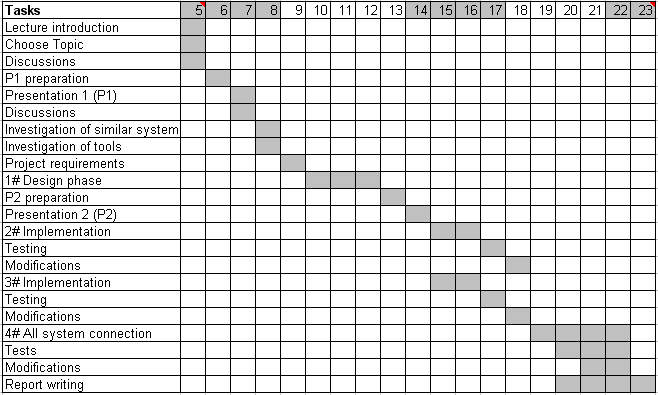
\includegraphics[scale=0.7]{planning}
	\caption{Work flow (Gant chart)}
	\label{fig:planning}
\end{figure}

\newpage
Work flow divided into four phases:

\begin{enumerate}
  \item 1\# Design – drawing diagrams, talking about similar systems and tools
  \begin{enumerate}
    \item Entity relation (ER) diagram
    \item Database connection class diagram (MySQL library)
    \item Sorting algorithm diagram
    \item Socket transfer protocol specifications
  \end{enumerate}
  \item 2\# Implementation
  \begin{enumerate}
    \item Configuration of database server
    \item Implementation of MySQL libraries
    \item Configuration of Web server
    \item Sorting algorithm
  \end{enumerate} 
  \item 3\# Implementation
  \begin{enumerate}
    \item Socket transfer server
    \item Sorting algorithm
  \end{enumerate}
  \item 4\# All system connection - all part connection into one software
  \begin{enumerate}
    \item Control RFID reader and provide access to subtask 4
    \item Connect RFID reader with sorting algorithm
    \item Connect RFID reader with socket transfer server
    \item Connect all together: RFID reader, MySQL library, socket transfer server and sorting algorithm
  \end{enumerate} 
\end{enumerate}

\newpage
\subsection{Work Responsibilities}


\begin{table}[h]
	\centering
    \begin{tabular}{ | p{3cm} | p{5cm} |}
    \hline
    \textbf{Responsibilities} &  \textbf{Tasks} \\ \hline
    All & Lecture introduction\\ \hline
    All & Choose Topic\\ \hline
    All & Discussions\\ \hline
    All & P1 preparation\\ \hline
    All & Presentation 1 (P1)\\ \hline
    All & Discussions\\ \hline
    All & Investigation of similar system\\ \hline
    All & Investigation of tools\\ \hline
    All & Project requirements\\ \hline
    All & 1\# Design phase\\ \hline
    All & P2 preparation\\ \hline
    All & Presentation 2 (P2)\\ \hline
    All & 2\# Implementation\\ \hline
    All & Testing\\ \hline
    All & Modifications\\ \hline
    All & 3\# Implementation\\ \hline
    All & Testing\\ \hline
    All & Modifications\\ \hline
    All & 4\# All system connection\\ \hline
    All & Testing\\ \hline
    All & Modifications\\ \hline
    All & Report writing\\ \hline
 		\end{tabular}
 		\caption{Work flow responsibilities}
	\label{tab:WorkFlow}
\end{table}


\subsection{Expectations}

To make sure that project will be delivered in time and all software function.

%
\section{Collaboration between subtasks}

The project requires collaboration between subtasks. Each subtask has its own knowledge area, requirements and expectations, however the subtasks are closely related. Our subtask is completely software orientated. The collaboration with the other subtask are described in the following subsections:

\subsection{Collaboration between subtask 4 and 5}
\begin{itemize}
	\item Requirements from task 4
	\subitem - Provide list of scanned clothes through defined protocol [Appendix A].
	\item Requirements to task 4
	\subitem - No requirements.
\end{itemize}

\subsection{Collaboration between subtask 6 and 5}
\begin{itemize}
	\item Requirements from sub task 6
	\subitem - Provide access to data base through created library.
	\item Requirements to task 6
	\subitem - Provide library of RFID readers.
\end{itemize}

\subsection{Collaboration between subtask 2 and 5}
\begin{itemize}
	\item Requirements from sub task 2
	\subitem - Allocate data base space to store data.
	\subitem - Created tables.
	\subitem - Provided general libraries.
	\subitem - Provided configuration tool.
\end{itemize}

During the project there were many meetings between groups to understand the project flow, complexity, find and solve any problems. Meetings and discussions were important to understand what is wrong and what is going well. The meetings were very productive, helped stay on schedule and accomplish our goals.
%
\section{Database design}

Around the world there are a lot of different types of databases \cite{bib1}. We have chosen to use MySQL, the most popular - relational database. Relational databases are easy to understand \cite{bib2} and use. Relational databases are collections of relations, this organization and structure of the data set meets our requirements, and can be used for our project.

\subsection{Why MySQL?}

There are many different relational databases [3] and choosing one can be difficult. Our choice was MySQL database, because it is:

\begin{itemize}
	\item Open source database
	\item Ease to use
	\item Fast performance
	\item Reliable 
	\item Most popular open source DB in the world
	\item It is used by Yahoo!, Alcatel-Lucent, Google, Nokia, YouTube and many others
\end{itemize}

\subsection{ER diagram}

Design of the database starts at the modeling phase. One of the most popular approaches is conceptual modeling, using entity relational diagram (ER) \cite{bib4}. Entity relational diagrams shows collections of relations in the modeling database. ER diagram makes it easy understand the concept of the database. Another methodology to model databases is UML diagrams. Most OOP programmers are familiar with UML. In the modeling and design phases ER diagrams was used and later it were converted to UML [Appendix B].

\begin{figure}[h]
	\centering
		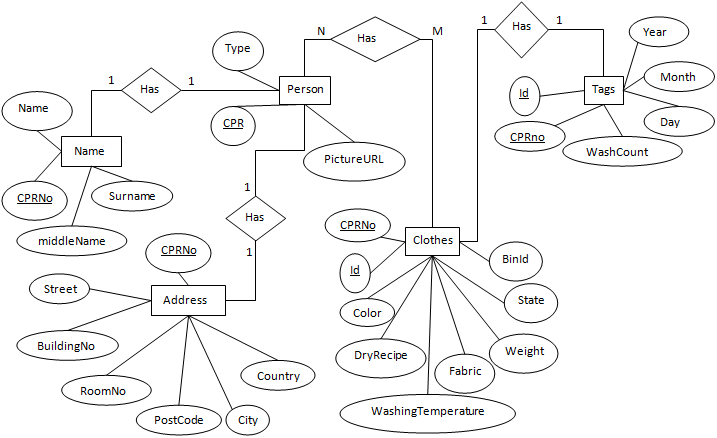
\includegraphics[scale=0.7]{erDiagramSmall}
	\caption{Laundry ER diagram}
	\label{fig:planning}
\end{figure}

\subsection{Implementation}

Before making the database it is needed to create tables and move them into database. Database tables were created by using a query language like shown in the figure \ref{fig:personAndNamesTable}. All the code was written into a text file and the text file was uploaded directly to database by using the created configurator tool.

\begin{figure}[h]
	\centering
		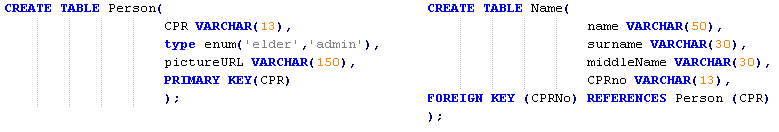
\includegraphics[scale=0.6]{personAndNamesTable}
	\caption{Person and Name tables}
	\label{fig:personAndNamesTable}
\end{figure}

The person table has three attributes: CPR, type and pictureURL and primary key for CPR. The primary key makes table unique, without a key the table would become a weak entity type, note that it is always good to have tables with strong entity types \cite{bib4}. Foreign key makes table name also unique. The table name has one unique reference to the person table and the person table is unique. \\ A configurator was created to make it easy to management the database, which is able connect to database and configure by a query language or send files with configuration sentences. This makes it faster to update and change without the need of writing database code. 

\subsection{Future work}

The usage of all tables is not optimal and/or optimized and some attributes can be unnecessary and are not used at all, the space usage can be decreased. The system has not been design with speed considerations in mind and the speed can be increased.
%
\section{Laundry data base library}

Mostly of the project subtasks decided to use one programming language to make easy work together. Sometimes different languages can be difficult connect and work together. That is why decided to use one object oriented language – C\#. As we know C\# is a new generation language which provides a lot of advance features like garbage collector and more others. This kind of language makes easier developer write programs, because here do not need take care about low level features like memory allocation or lost pointer. So this kind of language can decrease development process and increase code efficiency. \\
Our case design was to store and provide data about the elders. All data were stored in MySQL data base. So many of subtask would like to use it and that is why were decided to create general library for any to use. Main design requirement is to create general library which has features:  reliable, easy maintain, simple to use, and easy update.

\subsection{Design phase}

To keep above mentioned requirement and features, decided to create a DLL (dynamic link library) which can be executable and contain inside code, data, and resources. Our design library inside have two classes:

\begin{itemize}
	\item MySQLConnection – data base connector which responsible for connection to data base and send/receive queries.
	\item Functions – general library for laundry data base.
\end{itemize}

\begin{figure}[h]
	\centering
		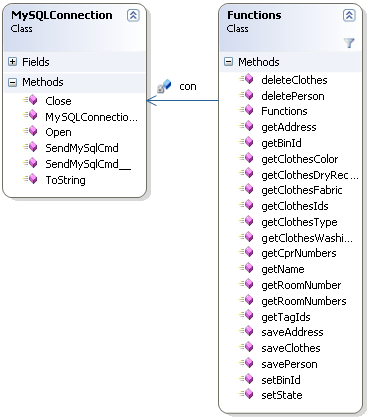
\includegraphics[scale=0.7]{classLibrary}
	\caption{Class library of the data base connection}
	\label{fig:planning}
\end{figure}

\newpage
\subsection{Implementation}

Software development was related to unified process (UP) – iterative incremental process.  Iterative incremental process model [5] was used during the implementation.  
Let us explain everything in more detail. Project were created using class Library in Microsoft Visual C\# .NET 3.5. To have data base connection were included MySQL Connector Net 1.0.10 into references. To use created library we need include it into new project (Console or Win or else) and start our library. For example we insert our library into console project, so connection to data base is like shown in the figure 6.1. After successful connection we can use class functions and manage laundry data base. 
\newpage
Numbers explain data base connection parameters: 

\begin{figure}[h]
	\centering
		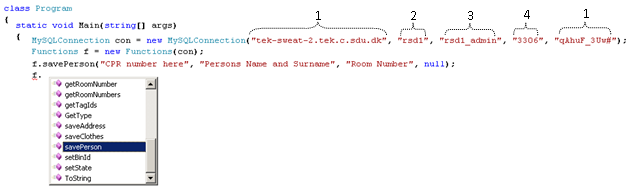
\includegraphics[scale=0.7]{connectionToData}
	\caption{Connection to data base server and save new person}
	\label{fig:planning}
\end{figure}

\begin{enumerate}
	\item IP address or domain
	\item Data base name
	\item User Id
	\item Port number
	\item Password
\end{enumerate}

Class functions uses created instance of MySQLConnection library. And throw the variable f can be connected to all created methods. At the figure 6.2 shows an example of creation new person. As we can see there used methods send queries to data base. New CPR inserted into table person by query: “INSERT INTO Person (CPR) Values (‘1234567890’)”.

\begin{figure}[h]
	\centering
		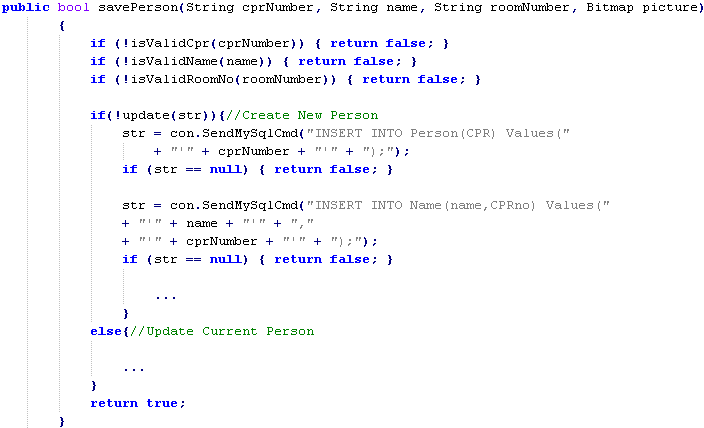
\includegraphics[scale=0.7]{exampleSavePerson}
	\caption{Example of save person method}
	\label{fig:planning}
\end{figure}

\subsection{Future work}
%
\section{Socket transfer server}

Another more general approach is to use socket communication [6] protocol. Many applications – from the networks to the mobile phones [7] use sockets. Designing software requirement is communicate with the clients and provide database information. Also keep multiple connections at the time and keep it simple.  Socket transfer server also like MySQLLIbrary was designed by using C\# programming language. It is reasonable to use one programming language during all project, therefore connection to other part be easier. \\ In general sockets very usable to use: 

\begin{itemize}
	\item Created socket transfer server and specified protocol can be used and understand by any programming language.
	\item Easy update and maintain new requirements only updates protocol specification, does not need to change server.
\end{itemize}

\subsection{Socket protocol specification}

To start design and implement our software we need to define protocol. Throw the protocol we communicate and change information. General protocol description showed in the table 7.1. Start command defines protocol type and always communication string start with 0xFE. Command type range allocated from 0x11 to 0x90, where is one byte describing command. The last one is value where is a content of data.

\begin{table}[h]
	\centering
    \begin{tabular}{ | p{4cm} | p{5cm} | p{4cm} | }
    \hline
    \textbf{Start Command} [0xFE] & \textbf{Command type} [0x11 - 0x90] & \textbf{Value}  \\ \hline
    1 byte & 1 byte & 4 or 24 bytes  \\ \hline
    \end{tabular}
	\caption{General protocol specification}
	\label{tab:protocolSpec}
\end{table}

\textbf{Example 7.1}: Subtask 4 wants to get a bin number for particular tag. So they sending string like this: 
"\textbf{0xFE 0x12} 0x30 0x30 0x30 0x30 0x31 0x32 0x33 0x34 0x31 0x32 0x33 0x34 0x41 0x41 0x31 0x32 0x33 0x34 0x35 0x36 0x41 0x34 0x35 0x36", where at the beginning defined protocol type and command type, rest of the hexadecimal values are tag id. If there are no errors in the string transfer server converts tag id to ASCII characters and sends constructed query to database. Response from database will be ASCII character which will be converted to hexadecimal and constructed packet send back to the client: "\textbf{0xFE 0x12} 0x00 0x00 0x00 0x00".

\begin{table}[h]
	\centering
    \begin{tabular}{ | p{1cm} | p{3cm} | p{3cm} | p{5cm} |}
    \hline
	& \textbf{Protocol type} & \textbf{Command type} & \textbf{Value}  \\ \hline
	Value & 0xFE & 0x12 & 000012341234AA123456A456 \\ \hline
	Bytes & 1 & 1 & 24  \\ \hline
    \end{tabular}
	\caption{Command packet (from client to server)}
	\label{tab:FromClient}
\end{table}

\begin{table}[h]
	\centering
    \begin{tabular}{ | p{1cm} | p{3cm} | p{3cm} | p{5cm} |}
    \hline
	& \textbf{Protocol type} & \textbf{Command type} & \textbf{Value}  \\ \hline
	Value & 0xFE & 0x12 & 0 \\ \hline
	Bytes & 1 & 1 & 4  \\ \hline
    \end{tabular}
	\caption{Command packet (from server to client)}
	\label{tab:FromServer}
\end{table}

\subsection{Design and implementation}

When protocol specified we can start design and implement software. Class diagram shown in the figure 7.1. \\ Here we can see four part:

\begin{enumerate}
	\item Starts server and stops main thread forever.
	\item Started server waiting for incomming packets. Incomming socket packet rises event.
	\item Transfered protocol opened and checked for incoming command. If command is not recognized then execution stoped and waiting for another incomming packet.
	\item Socket packet is class where defined buffer size, incoming client information.
\end{enumerate}

\begin{figure}[h]
	\centering
		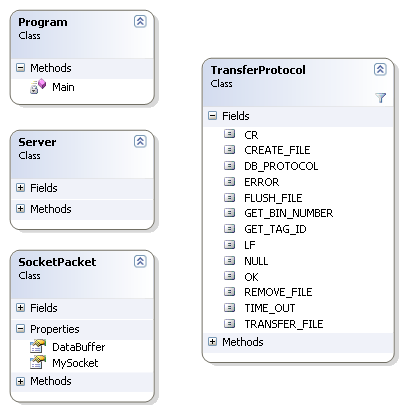
\includegraphics[scale=0.7]{socketClassDiagram}
	\caption{Class diagram of the socket transfer server}
	\label{fig:planning}
\end{figure}


\subsection{Future work}

In the future socket transfer server can be extended to have files transferring features and some security. File transferring protocol already defined however do not implemented. It could be used save elder picture. Security could be used to make safe transfer. However both of above mentioned features are not important. Picture is just additional feature and does not make sense to project. Security only necessary if transferring server will be placed out of the domain. In other case local LAN is already have security.
%
\section{Sorting algorithms}

All of us know that washing black and white together is a bad idea; however there are a lot of criteria to distinguish and prepare clothes for washing. This chapter presents several sorting algorithms for preparation to wash. 

\subsection{Requirements/criteria}

Mostly all of the clothes have the sewed label (tag). There are defined information about fabric, washing temperature and etc. For instance fabric defines the material of clothe –how clothe is sensitive.  For instance wool is more sensitive when synthetic or clothe which can be washed 40 degree is more sensitive than clothe which can be washed 95 degree. Of course sometimes 40 degree clothe can be washed on 30 or 60 degree and 95 degree can be washed on 60 degree temperature. \\ \\ A general criterion’s used to create sorting algorithm:

\begin{itemize}
	\item Colour – often there are bad idea wash white and black together, so this criteria defines that clothes of colored and white should be distinguished and washed separately. 
	\item Washing temperature – some clothes are more sensitive than other, so clothe should be washed on temperature defined by label in other case there could be possibility to damage clothe.
	\item Fabric – defines material of the clothes. For instance wool, cotton, synthetic and etc. All those material types have different sensitive criterions. Comparing wool and synthetic of the same color and temperature we should take in to account that wool is higher priority clothe and same synthetic clothe should be washed regarding rules of wool.
	\item Weight – defines bin size of washing machine size. In other words how many clothes can fit to washing machine and be washed.
\end{itemize}

\noindent Abstract criterion defines how clothes can be washed:

\begin{itemize}
	\item White and light clothes can be washed together
	\item Colored and dark clothes can be washed together
	\item Light, white and cotton often are washed on higher temperatures 60 degree or higher
	\item Cotton and wool can be washed together, however all rules set regarding wool
	\item Daily clothes temperatures around 60 degree
	\item Work clothes temperatures around 90 degree
	\item Washing temperature of wool is low (below 40 degree)
	\item Cotton more sensitive than synthetic
	\item Wool more sensitive than cotton
\end{itemize}

\subsection{Sorting algorithm designs}

\subsubsection{Sorting by color and temperature}

Algorithm presented in figure 8.1 is one of the simplest, which is also implemented. When list of clothes comes to sort, then each clothe are moved to particular bin. First are sorted by color and then by temperature. Number of total possible bins is ten – five for colored and five for white. Bins are numbered automatically.

\begin{figure}[h]
	\centering
		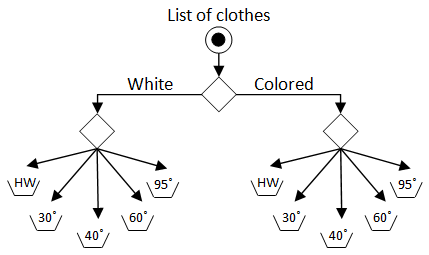
\includegraphics{sortingByColorTemp}
	\caption{Sorting algorithm by color and temperature}
	\label{fig:planning}
\end{figure}

This kind of algorithm is not optimal, because one clothe can be washed as well. Of course if time is not so important, then clothes from the bin should be washed when bin is full.

\subsubsection{Sorting algorithm using configurable parameters}

A lot of laundry institution sorting clothes similar but not the same. One of them has different size washing machines others wash at the higher temperature and all of them have distinct criteria’s.   So question is: how can be created software which satisfied all user requirements. \\  Here presented software based on C\# language, software consists of two parts: configuration and sorting algorithm. Configuration part is finished, however sorting algorithm do not finished. Purpose of the configuration is to save and load sorting criteria’s created by user. 

Each of clothe has sewed label which defines temperature, fabric and it would be great to prioritize clothes by sensitive. Purpose of that is to sort by priorities; more sensitive clothes have more privileges than low priority clothes. Same color and same washing temperature clothes could have different priorities, for instance one clothe is from wool and another from synthetic, so synthetic (possible) is lower priority than wool and should be washed considering wool. Clothes of the lower priority washed considering higher priority and highest priority washed like it have to be washed. Figure 8.1 (left) presents an example of configured priorities. Most significant clothes are in the top of list (example: Cotton: Hand wash: 95, Wool: Degree 30: 90) and have the highest priority and least significant down in the list. \\ Different institutions have different washing machine sizes, and all of them during one washing cycle want to utilize max clothes. That is why included parameters like total washing machine size and each clothe size figure 8.1 (right). Total washing machine size defines the threshold (in that case 87\%) which defines when is not optimal to wash. In other words washing machine utilization bellow 87\% is not optimal and can not be washed. Another configuration of size is how many units of particular type of clothe can fit in one washing machine. 


Last feature included is washing alternatives, in other words what to do then clothe can not be washed in particular case. Figure 8.2 presents alternatives of cotton: 30 degree. As we can see this kind of clothe can be washed with the wool: 30 degree (plan B) or Synthetic: 30 degree (plan C) or wool: 40 degree (worst plan if before two does not fit). Each clothes could have any size of plans. All above mentioned parameters can be saved, loaded or updated for the next time use. As we can see many features provides quite wide range of washing possibilities.

Further presented sorting algorithm which shown in the figure 8.3. There are four parts (Init, I, II, III) describing algorithm in more abstract level. There is one input for incoming clothes and three outputs for outgoing results of the sort. Incoming clothes have parameters like: color, washing temperature, clothe type and fabric and result is a bin designated to current clothe.  Let us explain those four parts in more detail:

\begin{itemize}
	\item 3. Init – all incoming clothes sorted by color and washing temperature. By default all clothes get bin ids and calculated current state. Current state – defines is sort is enough efficiency.
	\item 4. I – check for success. That part check is current state enough efficiency. If it is than algorithm stops, or emerge time out.
	\item 5. II – try to move clothes from rest to reserve using washing alternative rules. 
	\item 6. III – try to decrease number of clothes. For example at the table 8.1 rows two and nine utilization is the same 818\%, however efficiency is different. One uses 8 bins and not efficiency another pass then uses 9 bins (times to be washed).
\end{itemize}

\begin{figure}[h]
	\centering
		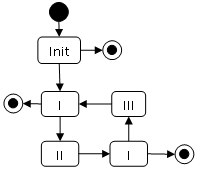
\includegraphics{sortingAlgorithm}
	\caption{Sorting algorithm}
	\label{fig:planning}
\end{figure}

Loop is going I, II, I, III, I... while do not get efficiency greater than 87\% (like set in configuration). By default if there are no configurations set, then algorithm works like presented in above chapter (sorting by color and temperature).

\begin{table}[h]
	
    \begin{tabular}{ | p{0.4cm} | p{1cm} | p{2cm} | p{1.7cm} |p{2cm} |p{1cm} |p{1.3cm} |p{1.2cm} |p{1.3cm} |}
    \hline
	Bin Id & Color & Washing Temperature & TotalBin Utilization (TBU) & NumberOf Bins Require (NBR) & Rest & Efficiency & Reserve & Success\\ \hline
	1 & White & 95 & 448\% & 4 & 48\% & 48\% & 52 \% & Fail \\ \hline
	2 & White & 60 & 818\% & 8 & 18\% & 18\% & 82 \% & Fail \\ \hline
	3 & White & 40 & 89\% & 1 & 0\% & 89\% & 11 \% & Pass \\ \hline
	4 & White & 30 & 639\% & 6 & 39\% & 39\% & 61 \% & Fail \\ \hline
	5 & White & HW & 159\% & - & - & - & - & - \\ \hline
	6 & Colored & 95 & 698\% & 7 & 0\% & 99\% & 2 \% & Pass \\ \hline
	7 & Colored & 60 & 2110\% & 21 & 10\% & 10\% & 90 \% & Fail \\ \hline
	8 & Colored & 40 & 788\% & 8 & 0\% & 98.5\% & 1.5 \% & Pass \\ \hline
	9 & Colored & 30 & 818\% & 9 & 0\% & 90.8\% & 9.2 \% & Pass \\ \hline
	10 & Colored & HW & 420\% & - & - & - & - & - \\ \hline
	11 & ... & ... & ... & ... & ... & ... & ... & ... \\ \hline
	- & - & - & - & - & - & Total: 62.54\% & - & All: No \\ \hline
    \end{tabular}
	\caption{Example of current state (when: Total washing machine value 87 \%)}
	\label{tab:AdDis}
\end{table}

Current state of the sorting is respresented by table where all values mutate during sort. Quantity of incomming clothes set bin ids and total bin utilization (TBU). TBU – how many times need to be washed it calculated by 8.1 formula:

Where clothe type can be: Sweater, Shirt, Pants, Underwear, WashingBag, Dress, Shorts, Towel and BedLinen. 



Efficiency can be calculated considering rest, diagram shown in figure 8.4. Efficiency describes is there cost-efficiency to wash or not. Wash is cost efficient than efficiency is greater 87\%.


\begin{figure}[h]
	\centering
		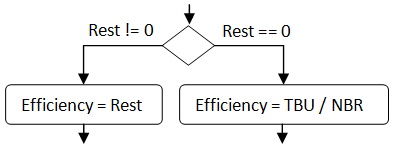
\includegraphics{efficiencyCalculation}
	\caption{Efficiency calculation diagram}
	\label{fig:planning}
\end{figure}

At the beginning incoming clothes are toke one after another and moved to the particular bin. If there are no clothes left than check how many distinct bins require. If there are more than zero bins than calculated and set current state like shown in the 8.1 table. If there are no clothes therefore there are no bins and algorithm is ended.

\begin{figure}[h]
	\centering
		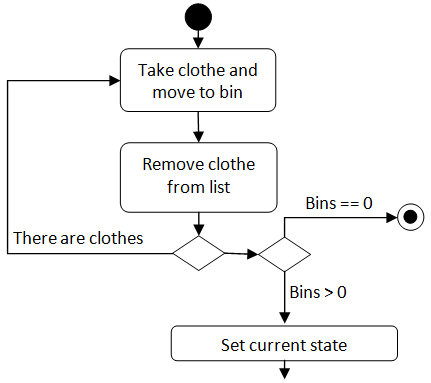
\includegraphics{diagramInit}
	\caption{Diagram Init}
	\label{fig:planning}
\end{figure}


Second move of algorithm is check for success and for time-out, figure 8.6. If all bins are greater efficiency than 87\% than current state is satisfied and clothes can be washed. In other case there is time-out algorithm also stopped. Purpose of the time-out added to avoid infinitive loop.

\begin{figure}[h]
	\centering
		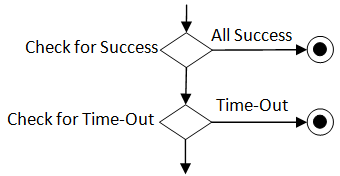
\includegraphics{diagramI}
	\caption{Diagram I}
	\label{fig:planning}
\end{figure}

Last two moves are very similar. Both of them try something to change when estimate current state and compare with previous. If new state is better than previous then state is set to current, in other case keep the last state. 

\begin{figure}[h]
	\centering
		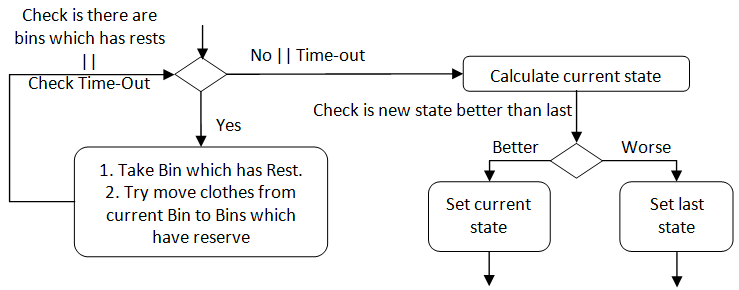
\includegraphics{diagramII}
	\caption{Diagram II}
	\label{fig:planning}
\end{figure}

At the figure 8.6 sorting algorithm trying to change the current state by moving clothes from bins which have rests to bins which have reserves and if result is better then new state set to current. 

\begin{figure}[h]
	\centering
		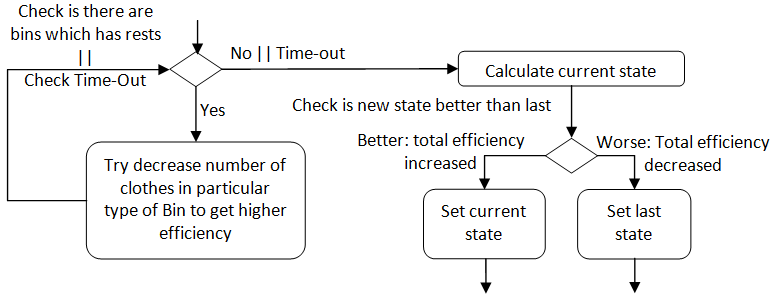
\includegraphics{diagramIII}
	\caption{Diagram III}
	\label{fig:planning}
\end{figure}

At the figure 8.7 sorting algorithm trying to change number of clothes in particular type of bin. For instance quantity of 818\% gives result for 8 bins and 18\% rest. However efficiency of 8 bins is 100\% and for the last one is only 18\%. Eight bins can be washed however the rest should be wait. So if there will be decreased number of clothes during one wash then could be increased efficiency. If 818\% of clothes we wash by 9 bins then we get efficiency of 90.8\% and reserve 9.2\%. So this is optimal and new state is set.

As we can see there are concurrency between II and III. If something changed at II then III have also possibilities to change and vice versa. Concurrency is essential to get a progress and mutation of states.
%
\section{Entire System Integration}

To make sure that all parts work, need connect them all to one software mechanism or control flow goes throw one point. Other case design could be multi agent systems (MAS) where all software will be separate agent.

Sorting algorithm, RFID reader, MySQL Library, socket transfer server

\begin{figure}[h]
	\centering
		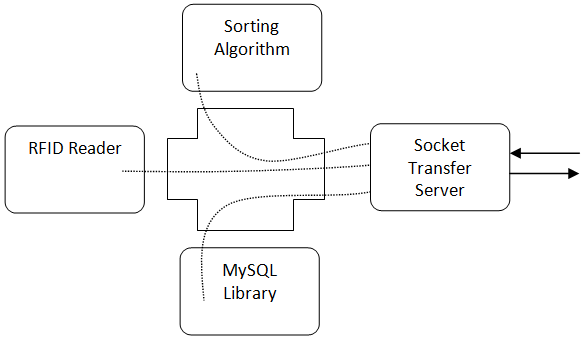
\includegraphics[scale=0.6]{softwareInteraction}
	\caption{Interaction between the different elements}
	\label{fig:planning}
\end{figure}


\subsection{Tests/Analysis/Functionality}

\begin{table}[h]
	
    \begin{tabular}{ | p{0.5cm} | p{3.5cm} | p{1.6cm} | p{1.6cm} |p{1.6cm} |p{1.6cm} |p{1cm} |}
    \hline
	No &  & Audrius Palisaitis & Kalle Grafstrom & Martin Moghadam & Robertas Jacauskas & Total\\ \hline
	1 & Data base & 100\% & 100\% & 100\% & 100\% & 100\% \\ \hline
	2 & MySQL library &  &  &  & 90\% &  \\ \hline
	3 & Socket Transfer server &  &  &  & 70\% &  \\ \hline
	4 & RFID reader &  &  &  & \% &  \\ \hline
	5 & Sorting Algorithm &  &  &  & 70\% &  \\ \hline
    \end{tabular}
	\caption{Estimation in percents of current system)}
	\label{tab:AdDis}
\end{table}

\begin{enumerate}
	\item Data base function very well, no errors during period
	\item MySQL library function well, however some exceptions during project period. Problems with MySQL connector library. Assumption that exceptions comes than some one tries to change data base during usage or problems with multithreading.
	\item Socket transfer server functions OK, however do not tested for 100\% and could be errors.
	\item RFID reader works OK, do not tested at all this is library taken from other group
	\item Sorting algorithm works OK, however do not tested for 100\%.
\end{enumerate}

\subsection{Future Work}

\begin{figure}[h]
	\centering
		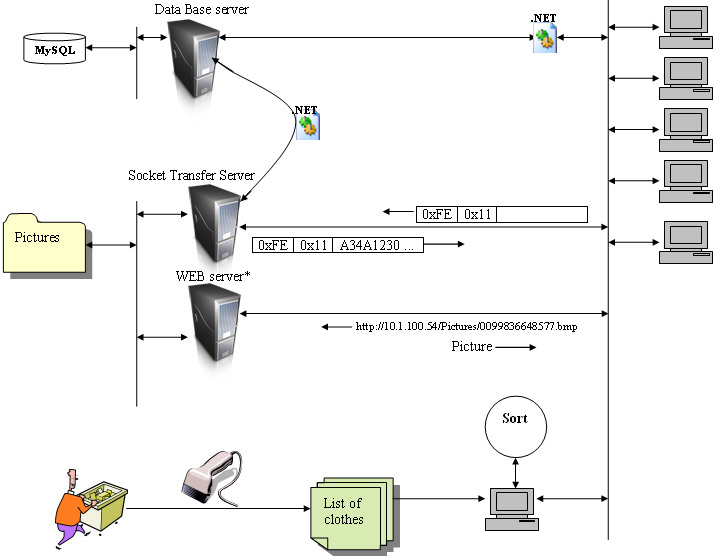
\includegraphics[scale=0.5]{entireSystem}
	\caption{Future System}
	\label{fig:planning}
\end{figure}
% Conclusion
\section{Conclusion}



%=======================================       

% Creates entry in bibliography even if it isn't cited.
\nocite{bib1} 
\nocite{bib2}

\bibliographystyle{unsrt} % references appear in order of citations
\bibliography{references}

\end{document}